\begin{zadatak} Nakon svake izvršene naredbe u primjerima i zadacima, izvršite naredbu \texttt{ls -l} kako bi vidjeli promjene.
\begin{itemize}
\item U direktoriju \texttt{vjezba7} kreirajte datoteku main.c u kojoj će biti neki c program.
\item Iskompajlirajte ga: \texttt{gcc -o main main.c} 
\item Napravite kopiju datoteke \texttt{main.c}. Neka se kopija zove \texttt{kopija.c}.
\end{itemize}
\end{zadatak}

\section*{Dozvole i vlasništvo datoteka i direktorija (\textit{file permission})}
\subsection*{Korisnici i grupe}
Da bi se datoteke zaštitile od neovlaštenog pristupa, Linux dozvoljava postavljanje dozvola korištenja datoteka i direktorija. Dozvole se određuju za:
\begin{itemize}
 \item vlasnika datoteke (\textbf{owner})
\item članove grupe kojoj je datoteka dodjeljena (\textbf{group})
\item sve ostale korisnike (\textbf{other}).
\end{itemize}
\begin{primjer} Izvršite \texttt{ls -l}. Prvih 10 znakova označava dozvole korištenja datoteke, zatim je broj koji označava broj linkova, sljedeća polja su vlasnik, grupa, veličina, 
vrijeme zadnje promjene i ime datoteke.

\lstinline!-rwxr-xr-x 1 os os 10103 2010-12-15 10:58 main !

\lstinline!-rw-r--r-- 1 os os   248 2010-12-15 10:58 main.c!
\end{primjer}
U gornjim primjerima:
\begin{itemize}
 \item Prvi znak \texttt{-} ili \texttt{d} označava tip datoteke (datoteka ili direktorij).
\item Sljedeća tri znaka \texttt{rwx} ili \texttt{rw-} označavaju dozvole vlasnika datoteke.
\item Sljedeća tri znaka \texttt{r-x} ili \texttt{r$--$} označavaju dozvole za grupu.
\item Sljedeća tri znaka \texttt{r-x} ili \texttt{r$--$} označavaju dozvole za ostale korisnike.
\end{itemize}
\textbf{Za datoteke:}\\
Troslovna kombinacija slova \texttt{r}, \texttt{w} i \texttt{x} označavaju redom pravo čitanja, pisanja i izvršavanja datoteke.\\
\textbf{Za direktorije:}
 \begin{itemize}
\item 
\texttt{r}: korisnik može vidjeti sadržaj direktorija (npr. sa \texttt{ls} naredbom).                                                                                                            
\item \texttt{w}: korisnik može mijenjati sadržaj direktorija tj. kreirati, brisati i preimenovati datoteke u direktoriju.
\item \texttt{x}: korisnik može koristit direktorij kao svoj tekući direktorij, tj. može ući u njega naredbom \texttt{cd}. 
\end{itemize}
\subsection*{Mijenjanje dozvola}
Sintaksa \texttt{chmod <MODE> <ime\_datoteke>}
\\
\texttt{<MODE>} može biti napisan simbolički npr. \texttt{chmod go-rx kopija.c} ili oktalno npr. \texttt{chmod 700 kopija.c}.\\
\subsubsection*{Simbolički}\texttt{chmod <TKO OPERATOR STO> <ime\_datoteke>}\\
\texttt{<TKO>} može biti:
\begin{itemize}
 \item \textbf{u} user
\item \textbf{g} grupa
\item \textbf{o} ostali
\item \textbf{a} svi
\end{itemize}
\texttt{<OPERATOR>} može biti:
\begin{itemize}
 \item \textbf{+} dodavanje prava
\item \textbf{-} oduzimanje prava
\item \textbf{=} skidanje svih prava i dodavanje specificiranih
\end{itemize}
\texttt{<STO>} može biti \textbf{r}, \texttt{w} i \textbf{x}.

\begin{primjer}{Primjer simboličkog načina pridjeljivanja prava korištenja:}
\begin{itemize}
 \item \texttt{chmod u=rw,go=r kopija.c} - user dobija pravo pisanja i čitanja, a grupa i ostali samo čitanja.
\item \texttt{chmod a+x main} - svi dobiju pravo izvršavanja uz već postojeća prava.
\end{itemize}
\end{primjer}
\subsubsection*{Oktalno zapisivanje prava korištenja}
\texttt{chmod <ZZZ> <ime\_datoteke>}\\
Z - oktalna znamenka (znamenka između 0 i 7)
%\begin{figure}
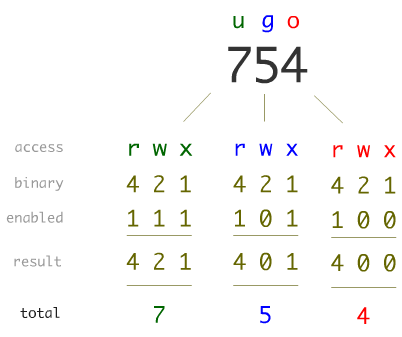
\includegraphics[scale=0.3]{07_File_perm_03.png}
%\end{figure}

\begin{primjer}Primjer oktalnog načina pridjeljivanja prava korištenja:
\begin{itemize}
 \item \texttt{chmod 644 kopija.c} - user dobija pravo pisanja i čitanja, a grupa i ostali samo čitanja.
\item \texttt{chmod 755 main} - svi dobiju pravo izvršavanja uz već postojeća prava.
\end{itemize}
\end{primjer}
\begin{zadatak}
Datoteci \texttt{kopija.c} dodijelite takva prava da samo \texttt{user} može mijenjati datoteku. 
\end{zadatak}
\begin{zadatak}
Datoteci \texttt{main} dodijelite takva prava da samo \texttt{user} i pripadajuća grupa mogu izvršavati datoteku tj. program \texttt{main}. 
\end{zadatak}
\begin{zadatak}
Datoteci \texttt{main} skinite pravo mijenjanja za \texttt{usera}. Pokušajte pokrenuti program \texttt{./main}. 
\end{zadatak}
\begin{zadatak}
Kreirajte direktorij \texttt{test} i u njega kopirajte datoteku \texttt{main}. Direktoriju \texttt{test} skinite pravo pisanja \texttt{w}. 
Kopirajte datoteku \texttt{main.c} u njega. Kakav je rezultat i zašto? 
\end{zadatak}

\begin{comment}

\vfill
\begin{itemize}
\renewcommand{\labelitemi}{\textbf{$\rightarrow$}}
\item Popis svih pokrenutih naredbi eksportirajte u datoteku imena \texttt{prezime\_ime\_vj7.txt}. Uploadajte datoteku na \href{https://moodle.oss.unist.hr/course/view.php?id=133}{http://moodle.oss.unist.hr}.
\end{itemize}

\end{comment}
